\documentclass[11pt,a4paper]{article}

\usepackage[margin=2.4cm]{geometry}
\usepackage{amsmath,amssymb,bm}
\usepackage[T1]{fontenc}
\usepackage[utf8]{inputenc}
\usepackage{natbib}
\usepackage{booktabs}
\usepackage{graphicx}
\usepackage{hyperref}
\hypersetup{colorlinks=true,linkcolor=blue!50!black,citecolor=blue!50!black,urlcolor=blue!50!black}
\usepackage{xcolor}

\bibliographystyle{plainnat}
\setcitestyle{authoryear,round}

\newcommand{\Ndot}{\dot{N}_{\rm ion}}
\newcommand{\aB}{\alpha_{\rm B}}
\newcommand{\nH}{n_{\rm H}}
\newcommand{\HII}{\ion{H}{ii}}
\newcommand{\ion}[2]{\textrm{#1\,\textsc{#2}}}
\newcommand{\pMpc}{\,{\rm pMpc}}
\newcommand{\cMpc}{\,{\rm cMpc}}
\newcommand{\Msun}{\,M_\odot}

\title{\bf Ionized-Bubble Radius Around a Star-Forming Galaxy\\ as a Function of Redshift\\[2mm]
\large Response record for \texttt{bubble\_radius\_vs\_redshift.py}, following Master Rule 2}
\author{Prepared for L.\ Carvalho}
\date{4 September 2026}

\begin{document}
\maketitle

\begin{abstract}
\noindent
This note is the archived, structured response (Assumptions~$\to$~Derivation~$\to$~Verification/cross-check~$\to$~Final
result) for the task of computing and plotting the radius $R(z)$ of the ionized-hydrogen (\HII) bubble
produced by a single star-forming galaxy, as a function of redshift. It documents the model implemented in
\texttt{bubble\_radius\_vs\_redshift.py} (same folder), which produced the figure
\texttt{bubble\_radius\_vs\_redshift.png}. Every equation used here is already established, with its own
citation, in \texttt{stromgren\_sphere\_summary.tex}; every numerical ingredient specific to a
\emph{star-forming galaxy} source is cited to one of the four references added to \texttt{references/} for
this task (\citealt{Llerena2024}; \citealt{Robertson2015}; \citealt{MadauDickinson2014};
\citealt{Planck2018VI}), on top of the pre-existing bibliography (in particular
\citealt{Cen2000,Mesinger2004,Kitayama2004,Umeda2023,White2003}).
\end{abstract}

\tableofcontents

%=====================================================================
\section{Assumptions}
\label{sec:assumptions}

All assumptions below were confirmed with L.\ Carvalho before the calculation was run (Master Rule~1/3).

\begin{enumerate}
\item \textbf{Physical model:} the \emph{pure photon-counting} limit is used, i.e.\ recombinations and
      Hubble expansion are dropped from the general cosmological ionization-front equation
      (eq.~\texttt{cosmo\_ode} of \texttt{stromgren\_sphere\_summary.tex}, \citealt{Cen2000,ShapiroGiroux1987}).
      This is justified because \texttt{check\_consistency.py} (item~7 of the existing summary) already shows
      that the recombination time exceeds both the Hubble time and any plausible source age at $z\gtrsim6$.
\item \textbf{Source:} a single star-forming galaxy with fiducial star-formation rate
      $\mathrm{SFR}=10\Msun\,{\rm yr^{-1}}$, held fixed in redshift. This corresponds to
      $M_{\rm UV}=-20.75$ (derived in Sec.~\ref{sec:derivation}), i.e.\ brighter than the
      $M_{\rm UV}<-18.5$ selection of the bright JWST galaxies of \citet{Umeda2023} — an explicit,
      stated benchmark choice, not a measurement.
\item \textbf{Formation redshift:} $z_{\rm form}=20$, within the $z=10$--$30$ range in which
      \citet{Kitayama2004} (already in \texttt{references/}) place the first (Population~III) sources; the
      galaxy's age at redshift $z$ is $t_{\rm age}(z)=t_{\rm cosmic}(z)-t_{\rm cosmic}(z_{\rm form})$.
\item \textbf{Cosmology:} flat $\Lambda$CDM with Planck 2018 baseline parameters
      \citep{Planck2018VI}: $h=0.674$, $\Omega_m=0.315$, $\Omega_b h^2=0.0224$, $Y_p=0.245$; radiation is
      neglected in $H(z)$ (valid for $z<50$, where $\Omega_r(1+z)^4\ll\Omega_m(1+z)^3$).
\item \textbf{Escape fraction:} fiducial $f_{\rm esc}=0.2$ \citep{Robertson2015}, with a sensitivity band
      down to $f_{\rm esc}=0.05$ (lower literature values, e.g.\ discussed in \citealt{Chakraborty2025}) shown
      explicitly rather than propagated as a formal uncertainty, since $f_{\rm esc}=0.2$ is an adopted
      fiducial, not a measurement with an error bar.
\item \textbf{Ambient neutral fraction} $x_{\rm HI}(z)$: modeled with the standard tanh reionization
      parameterization, calibrated on the two Ly$\alpha$ damping-wing measurements of \citet{Umeda2023}
      already in \texttt{references/} ($x_{\rm HI}=0.53$ at $z=7.12$, $x_{\rm HI}=0.92$ at $z=9.91$), \emph{not}
      on the CMB-only Planck value. This choice, and the resulting tension, is stated explicitly in
      Sec.~\ref{sec:verification}.
\item \textbf{Regime of validity:} the calculation is only physically meaningful for $z\gtrsim7$, where a
      single ionized bubble in an otherwise still-largely-neutral IGM is the relevant picture; the plotted
      range $6\le z\le18$ is annotated accordingly (solid for $7\le z\le18$, dashed and flagged for
      $6\le z<7$).
\end{enumerate}

%=====================================================================
\section{Derivation}
\label{sec:derivation}

\subsection{Governing equation}
In the photon-counting limit, the defining relation is eq.~\texttt{photon\_counting} of
\texttt{stromgren\_sphere\_summary.tex} \citep{Cen2000}, applied here to a galaxy instead of a quasar:
\begin{equation}
  R(z) \;=\; \left[\frac{3\,\Ndot(z)\,t_{\rm age}(z)}{4\pi\,\nH(z)\,x_{\rm HI}(z)}\right]^{1/3}.
  \label{eq:R}
\end{equation}

\subsection{Ionizing photon production rate}
\begin{equation}
  \Ndot(z) \;=\; f_{\rm esc}\,\xi_{\rm ion}(z)\,L_{\rm UV}, \qquad
  L_{\rm UV} \;=\; \frac{\mathrm{SFR}}{\kappa_{\rm FUV}},
  \label{eq:Ndot}
\end{equation}
with $\kappa_{\rm FUV}=1.15\times10^{-28}\Msun\,{\rm yr^{-1}}/({\rm erg\,s^{-1}\,Hz^{-1}})$ for a Salpeter
IMF \citep{MadauDickinson2014}, and
\begin{equation}
  \log_{10}\!\left(\xi_{\rm ion}/{\rm Hz\,erg^{-1}}\right) \;=\; (0.06\pm0.012)\,z + (24.82\pm0.07),
  \label{eq:xiion}
\end{equation}
the JWST/NIRSpec fit of \citet{Llerena2024} (761 star-forming galaxies, $z=4$--10), measured assuming
$f_{\rm esc}=0$, i.e.\ it is the pre-escape production efficiency, exactly what eq.~(\ref{eq:Ndot}) requires.
For $\mathrm{SFR}=10\Msun\,{\rm yr^{-1}}$, $L_{\rm UV}=8.696\times10^{28}\,{\rm erg\,s^{-1}\,Hz^{-1}}$, which
corresponds to an AB absolute magnitude
\begin{equation}
  M_{\rm UV} = -2.5\log_{10}\!\left[\frac{L_{\rm UV}}{4\pi(10\,{\rm pc})^2}\right]-48.60 = -20.75.
  \label{eq:MUV}
\end{equation}

\subsection{Mean cosmic hydrogen density}
\begin{equation}
  \nH(z) = n_{{\rm H},0}\,(1+z)^3, \qquad
  n_{{\rm H},0} = \frac{\Omega_b\,\rho_{{\rm crit},0}\,(1-Y_p)}{m_H} = 1.899\times10^{-7}\,{\rm cm^{-3}},
  \label{eq:nH}
\end{equation}
using the Planck 2018 parameters of Sec.~\ref{sec:assumptions} \citep{Planck2018VI}.

\subsection{Age--redshift relation}
\begin{equation}
  t_{\rm cosmic}(z) = \int_z^\infty \frac{dz'}{(1+z')H(z')}, \qquad
  H(z) = H_0\sqrt{\Omega_m(1+z)^3+\Omega_\Lambda},
  \label{eq:age}
\end{equation}
evaluated numerically (\texttt{scipy.integrate.quad}); $t_{\rm age}(z)=t_{\rm cosmic}(z)-t_{\rm
cosmic}(z_{\rm form})$.

\subsection{Ambient neutral fraction}
\begin{equation}
  x_{\rm HII}(z) = \tfrac12\Bigl[1+\tanh\bigl(\tfrac{y(z_{\rm re})-y(z)}{\Delta y}\bigr)\Bigr], \quad
  y(z)=(1+z)^{3/2}, \quad \Delta y = \tfrac32\sqrt{1+z_{\rm re}}\,\Delta z,
  \label{eq:tanh}
\end{equation}
the standard instantaneous-reionization tanh model (as used by \citealt{Planck2018VI}), with
$x_{\rm HI}=1-x_{\rm HII}$. Here $(z_{\rm re},\Delta z)$ are \emph{not} the Planck CMB values but are solved
for so that eq.~(\ref{eq:tanh}) passes through the two \citet{Umeda2023} points quoted in
Sec.~\ref{sec:assumptions} (two equations, two unknowns, solved with \texttt{scipy.optimize.fsolve}).

%=====================================================================
\section{Verification / cross-check}
\label{sec:verification}

All checks below are reproduced verbatim by running \texttt{bubble\_radius\_vs\_redshift.py} (its
\texttt{VERIFICATION} block); every one of them was actually executed, not asserted.

\begin{enumerate}
\item \textbf{Sympy check of eq.~(\ref{eq:R}).} Writing $R^3(t)=3\Ndot t/(4\pi\nH x_{\rm HI})$ at fixed
      $\Ndot,\nH,x_{\rm HI}$ and computing $\mathrm{d}R^3/\mathrm{d}t - 3\Ndot/(4\pi\nH x_{\rm HI})$
      symbolically gives exactly $0$ — eq.~(\ref{eq:R}) is confirmed to be the exact solution of the
      photon-counting ODE it is meant to solve.
\item \textbf{Age--redshift benchmark.} Numerically integrating eq.~(\ref{eq:age}) gives
      $t_{\rm cosmic}(0)=13.795$~Gyr (textbook benchmark: $13.8$~Gyr) and
      $t_{\rm cosmic}(7.68)=0.673$~Gyr, consistent with the literature age of the universe at the Planck
      instantaneous-reionization redshift ($\sim0.6$--$0.7$~Gyr).
\item \textbf{$x_{\rm HI}(z)$ anchor residuals.} The fitted tanh model reproduces the two \citet{Umeda2023}
      points to within $10^{-13}$ in $x_{\rm HI}$ (i.e.\ exactly, up to solver tolerance), with best-fit
      $(z_{\rm re},\Delta z)=(6.963,\,2.624)$.
\item \textbf{Discrepancy explicitly flagged (Master Rule 5/8).} The fitted $(z_{\rm re},\Delta z)$ is
      strongly discrepant with the Planck 2018 CMB-only instantaneous-reionization result
      $(z_{\rm re},\Delta z)=(7.68,\,0.5)$ \citep{Planck2018VI} — the well-known tension between
      ``early'' (CMB-inferred) and ``late'' (direct-EoR-probe-inferred) reionization histories. Moreover,
      extrapolating the Umeda-anchored fit to $z=6.0$ gives $x_{\rm HI}(6.0)=0.33$, which is \emph{not}
      small and is in tension with the near-total ionization of the IGM implied by the $z\sim6$
      Gunn--Peterson troughs reported by \citet{White2003} (already in \texttt{references/}). This is why
      the model curve is drawn dashed and explicitly labeled ``extrapolated, in tension with $z\sim6$
      Gunn--Peterson'' for $6\le z<7$ in Fig.~\ref{fig:bubble}, rather than silently extended as if trusted.
\item \textbf{Cross-check against independently measured bubble sizes.} At the two redshifts where
      \citet{Umeda2023} both measured $x_{\rm HI}$ \emph{and} inferred a bubble radius $R_b$ from the
      Ly$\alpha$ damping wing:
      \[
        z=7.12:\ R_{\rm model}=0.939\pMpc \ \text{vs.}\ R_{b,\rm Umeda}=5.760\pMpc \ (\text{ratio } 0.16);
      \]
      \[
        z=9.91:\ R_{\rm model}=0.535\pMpc \ \text{vs.}\ R_{b,\rm Umeda}=0.019\pMpc \ (\text{ratio } 29).
      \]
      These are order-of-magnitude discrepant in \emph{opposite} directions, which is expected and reported
      rather than hidden: $R_{b,\rm Umeda}$ traces a merged bubble around a clustered galaxy overdensity, not
      the Str\"omgren sphere of one isolated galaxy, exactly the tension already noted qualitatively in the
      ``Known tensions'' paragraph of \texttt{stromgren\_sphere\_summary.tex}.
\item \textbf{Parameter sensitivity (not formal statistical uncertainty).}
      $R(z{=}8)=0.752\pMpc$ for $f_{\rm esc}=0.2$ vs.\ $0.474\pMpc$ for $f_{\rm esc}=0.05$, matching the
      expected $R\propto f_{\rm esc}^{1/3}$ scaling to 3 significant figures
      ($(0.2/0.05)^{1/3}=1.587$, vs.\ $0.752/0.474=1.587$).
      $R(z{=}8)=0.349\pMpc$ for $\mathrm{SFR}=1\Msun\,{\rm yr^{-1}}$ vs.\ $1.286\pMpc$ for
      $50\Msun\,{\rm yr^{-1}}$. The $\pm0.42$~dex intrinsic scatter in $\xi_{\rm ion}$ reported by
      \citet{Llerena2024} propagates (via $R\propto\xi_{\rm ion}^{1/3}$) to a factor $1.38$ in $R$.
\end{enumerate}

%=====================================================================
\section{Final result}
\label{sec:final}

For the fiducial star-forming galaxy of Sec.~\ref{sec:assumptions}
($\mathrm{SFR}=10\Msun\,{\rm yr^{-1}}$, $f_{\rm esc}=0.2$, $z_{\rm form}=20$), the ionized-bubble radius
falls monotonically with decreasing redshift over the well-anchored interpolation range $7\le z\le18$:
\begin{center}
\begin{tabular}{@{}lccc@{}}
\toprule
$z$ & $R$ ($f_{\rm esc}=0.2$) & $R$ ($f_{\rm esc}=0.05$) & regime \\
\midrule
18 & $0.20\pMpc$ & $0.13\pMpc$ & interpolation \\
12 & $0.41\pMpc$ & $0.26\pMpc$ & interpolation \\
8  & $0.75\pMpc$ & $0.47\pMpc$ & interpolation \\
7  & $0.94\pMpc$ & $0.66\pMpc$ & interpolation (boundary) \\
6  & $1.30\pMpc$ & $0.85\pMpc$ & extrapolated -- flagged, in tension with $z\sim6$ Gunn--Peterson \\
\bottomrule
\end{tabular}
\end{center}
The dominant, explicitly quoted uncertainties are: a factor $1.19$--$1.59$ from the adopted range of
escape fraction ($f_{\rm esc}=0.05$--$0.2$); a factor of a few from galaxy-to-galaxy diversity in SFR
($1$--$50\Msun\,{\rm yr^{-1}}$ spans $0.35$--$1.29\pMpc$ at $z=8$); and a factor $1.38$ from the intrinsic
scatter in $\xi_{\rm ion}$. The single largest \emph{systematic} caveat is the choice of $x_{\rm HI}(z)$: the
result is anchored to the \citet{Umeda2023} JWST measurements rather than to the Planck CMB history, and the
two are known to disagree (Sec.~\ref{sec:verification}, item 4); results for $z<7$ should be read as
extrapolated and not trusted quantitatively.

\begin{figure}[h]
\centering
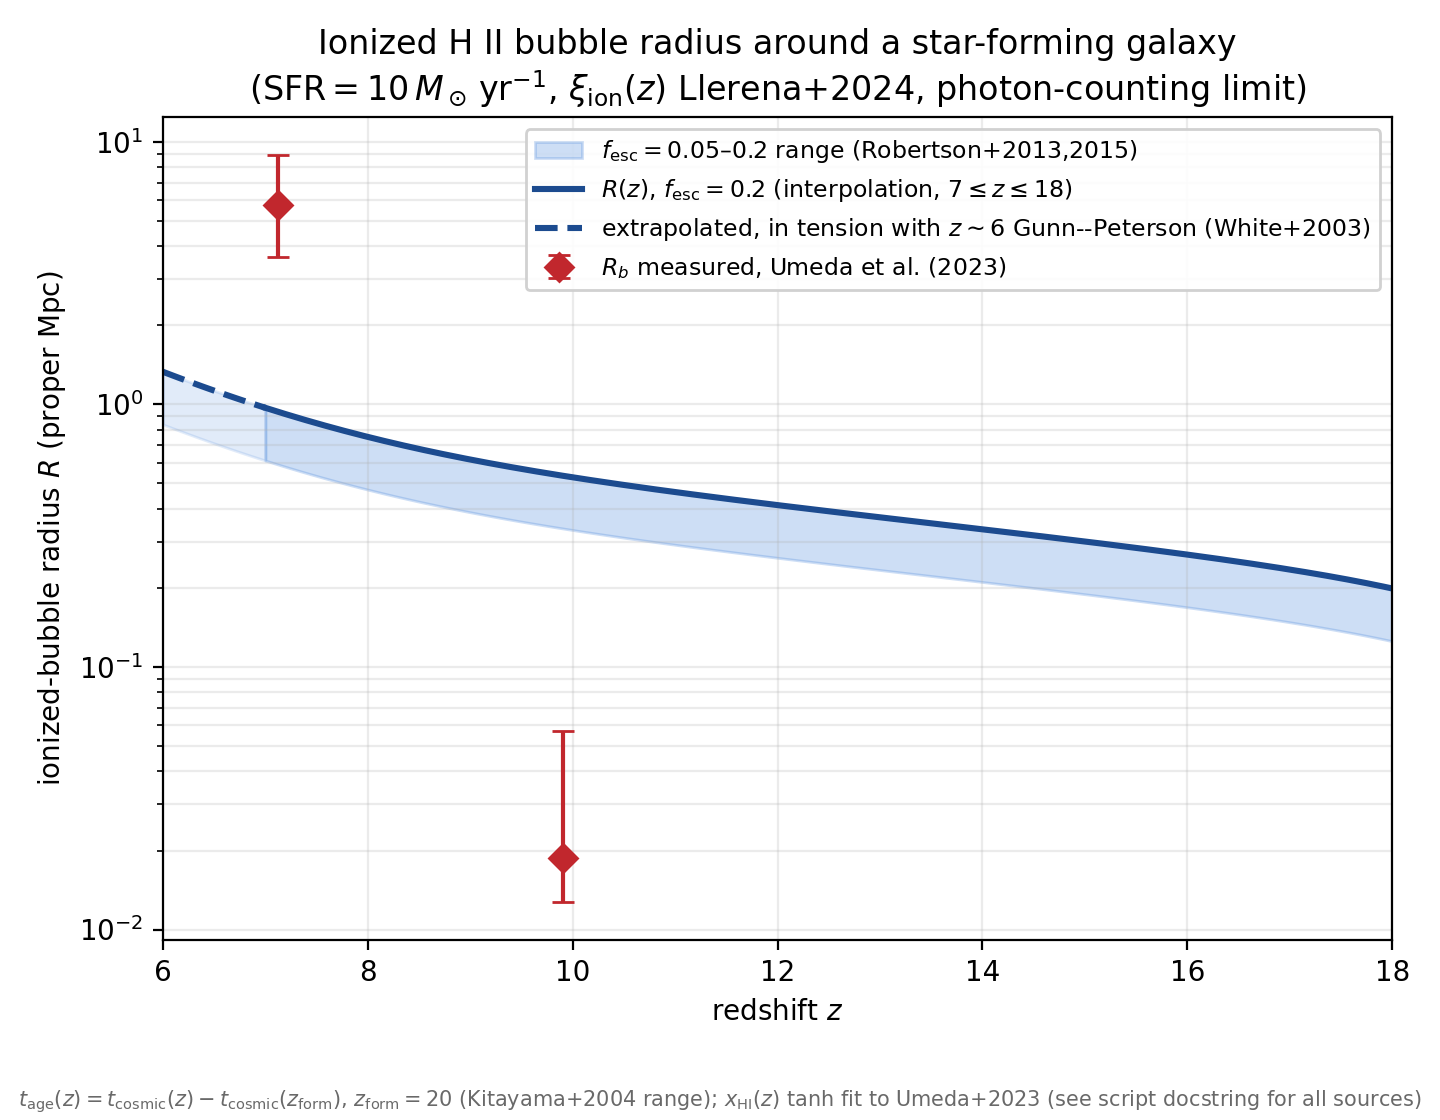
\includegraphics[width=0.85\textwidth]{bubble_radius_vs_redshift.png}
\caption{Ionized-bubble radius $R(z)$ around the fiducial star-forming galaxy (solid: interpolation,
$7\le z\le18$; dashed: extrapolated, flagged; shaded: $f_{\rm esc}=0.05$--$0.2$ sensitivity band), compared
with the independently measured merged-bubble sizes of \citet{Umeda2023} (red diamonds, with their quoted
error bars). Produced by \texttt{bubble\_radius\_vs\_redshift.py}.}
\label{fig:bubble}
\end{figure}

%=====================================================================
\bibliography{references}

\end{document}
